\clearpage
\raggedbottom
\phantomsection
\label{sec:appendix}
\etocdepthtag.toc{main}
\etocdepthtag.toc{appendix}

\vspace{0.8cm}
\begingroup
  \hypersetup{linkcolor=black}
  \color{black}
  \etocsettagdepth{main}{none}
  \etocsettagdepth{appendix}{subsection}
  \etocsettocstyle{\centering\bfseries {\Large Table of Contents}\par
    \vspace{0.1\baselineskip}
    \hrule
    \vspace{0.4\baselineskip}
  }{\vspace{0.4\baselineskip}
    \hrule height 0.4pt
  }
  \tableofcontents
\endgroup
\vspace{0.8\baselineskip}

\section{Appendix Overview}
This appendix covers the \ourmethod algorithm~(\cref{app:algo}), experimental details~(\cref{app:exp-details}), experimental results~(\cref{app:extended-results}), how the meta-agent modified the code~(\cref{app:evaluator-evolution}), the theory~(\cref{app:proofs}), and the limitations of our work~(\cref{app:limitations}).


\section{The Algorithm in Full}
\label{app:algo}

\Cref{alg:main} states the full \ourmethod{} procedure of \cref{sec:method}. Lines 1--4 initialize the frozen-epoch archive from the seed workspace $a_0$: every evaluator slot is set to its first epoch, frozen on its incumbent, and the seed is train-evaluated for lineage evidence only. Lines 5--21 run the inherited \cmp-guided search between checkpoints. At each iteration, the expansion gate (line 9) either expands or evaluates: an expansion samples a parent clade by metaproductivity (line 10), edits its workspace into a child (line 11), and admits the valid child to the archive with its own lineage-only train evaluation (lines 12--15); the iteration then samples a node by \cmp (line 17), picks its least-measured role--task cell (line 18), spends one unit of validation budget on that cell under the frozen evaluators (line 19), and records the binary outcome (line 20). Lines 22--31 run only at a checkpoint, the only point an evaluator can change. For each slot, the incumbent and its challengers are scored by the $\epsilon$-best-belief lower bound on evaluator-independent anchor counts (lines 24--25), and the highest is promoted with ties won by the incumbent (line 26); on a real change (line 27), the slot advances its epoch, freezes the new evaluator, erases the displaced slot's records, and recomputes the metaproductivity statistics (lines 28--29). Finally, lines 33--35 return the archive node with the highest $\epsilon$-best-belief score.

\makeatletter
\ifpaper@twocolumn
  \begin{algorithm*}[t]
\else
  \begin{algorithm}[t]
\fi
\DontPrintSemicolon
\LinesNumbered
\SetAlgoLined
\SetNlSty{textbf}{\scriptsize}{}
\SetAlgoNlRelativeSize{-1}
\footnotesize
\KwIn{Seed workspace $a_0$; roles $\mathcal R$; validation budget $B$; evaluator slots $1{:}M$}
\KwIn{Anchor sets $\mathrm{GT}[m]$; checkpoints $\mathcal C$; caps $(\bar B_{\rm exp},\bar B_{\rm train},\bar B_{\rm val})$; best-belief level $\epsilon$}
\KwOut{Archive $\mathcal T_B$ and selected endpoint agent $a^\star$}
\BlankLine
\textbf{Initialize the frozen-epoch archive.}\;
$\mathcal T \leftarrow \{a_0\}$; $N \leftarrow 0$; $j[m]\leftarrow 1$ for all slots $m$\;
$E[m]\leftarrow \func{Freeze}(\func{Incumbent}(m))$ for all slots $m$\;
$\func{TrainEval}(a_0,\mathcal R,E,\bar B_{\rm train})$\tcp*{lineage evidence only}
\BlankLine
\textbf{Run CMP-guided search between checkpoints.}\;
\While{$N < B$}{
  $b \leftarrow \min\{c\in\mathcal C:c>N\}\wedge B$\tcp*{next checkpoint}
  \While{$N < b$}{
    \If{$\func{ExpandGate}(\mathcal T,N)$}{
      $a_p \leftarrow \func{SampleCladeByCMP}(\mathcal T)$\;
      $a' \leftarrow \func{EditWorkspace}(a_p,\mathcal T,\bar B_{\rm exp})$\;
      \If{$\func{Valid}(a')$}{
        $\mathcal T \leftarrow \mathcal T \cup \{a'\}$\;
        $\func{TrainEval}(a',\mathcal R,E,\bar B_{\rm train})$\tcp*{not search utility}
      }
    }
    $a \leftarrow \func{SampleCladeByCMP}(\mathcal T)$\tcp*{node-level \hgm choice}
    $(r,d) \leftarrow \func{LeastMeasuredCell}(a,\mathcal R)$\tcp*{role/task balancing}
    $o \leftarrow \func{ValEval}(a,r,d,E,\bar B_{\rm val})$\;
    $\func{AddUtilityRecord}(\mathcal T,a,r,d,o,\mathbf j)$; $N \leftarrow N+1$\;
  }
\BlankLine
  \textbf{At checkpoint, replace evaluators only by anchor best-belief.}\;
  \ForEach{evaluator slot $m$}{
    $\Gamma_m \leftarrow \{E[m]\}\cup \func{Challengers}(m,\mathcal T)$\;
    $\mathrm{BB}[e] \leftarrow I_\epsilon^{-1}(1+S_e^{\rm gt},1+F_e^{\rm gt})$ for each $e\in\Gamma_m$\;
    $e^\star \leftarrow \func{Best}(\Gamma_m,\mathrm{BB};\ \func{tie}=E[m])$\;
    \If{$e^\star \neq E[m]$}{
      $j[m]\leftarrow j[m]+1$; $E[m]\leftarrow \func{Freeze}(e^\star)$\;
      $\func{EraseSlotRecords}(\mathcal T,m)$; $\func{RecomputeCMPStats}(\mathcal T)$\;
    }
  }
}
\BlankLine
\textbf{Select the endpoint by best-belief over archive nodes.}\;
$a^\star \leftarrow \func{BestBeliefNode}(\mathcal T,\epsilon)$\;
\Return{$(\mathcal T_B,a^\star)$}\;
\caption{\small Red Queen G\"odel Machine search with anchor-only evaluator replacement.}
\label{alg:main}
\ifpaper@twocolumn
  \end{algorithm*}
\else
  \end{algorithm}
\fi
\makeatother


\section{Experimental Setup}
\label{app:exp-details}

\subsection{Domains and Anchor pairs}

\Cref{fig:domain-utilities} shows how each domain pairs a generator role with a learned evaluator role and a \emph{ground-truth anchor}. 

\begin{widefigure}[tb]
\centering


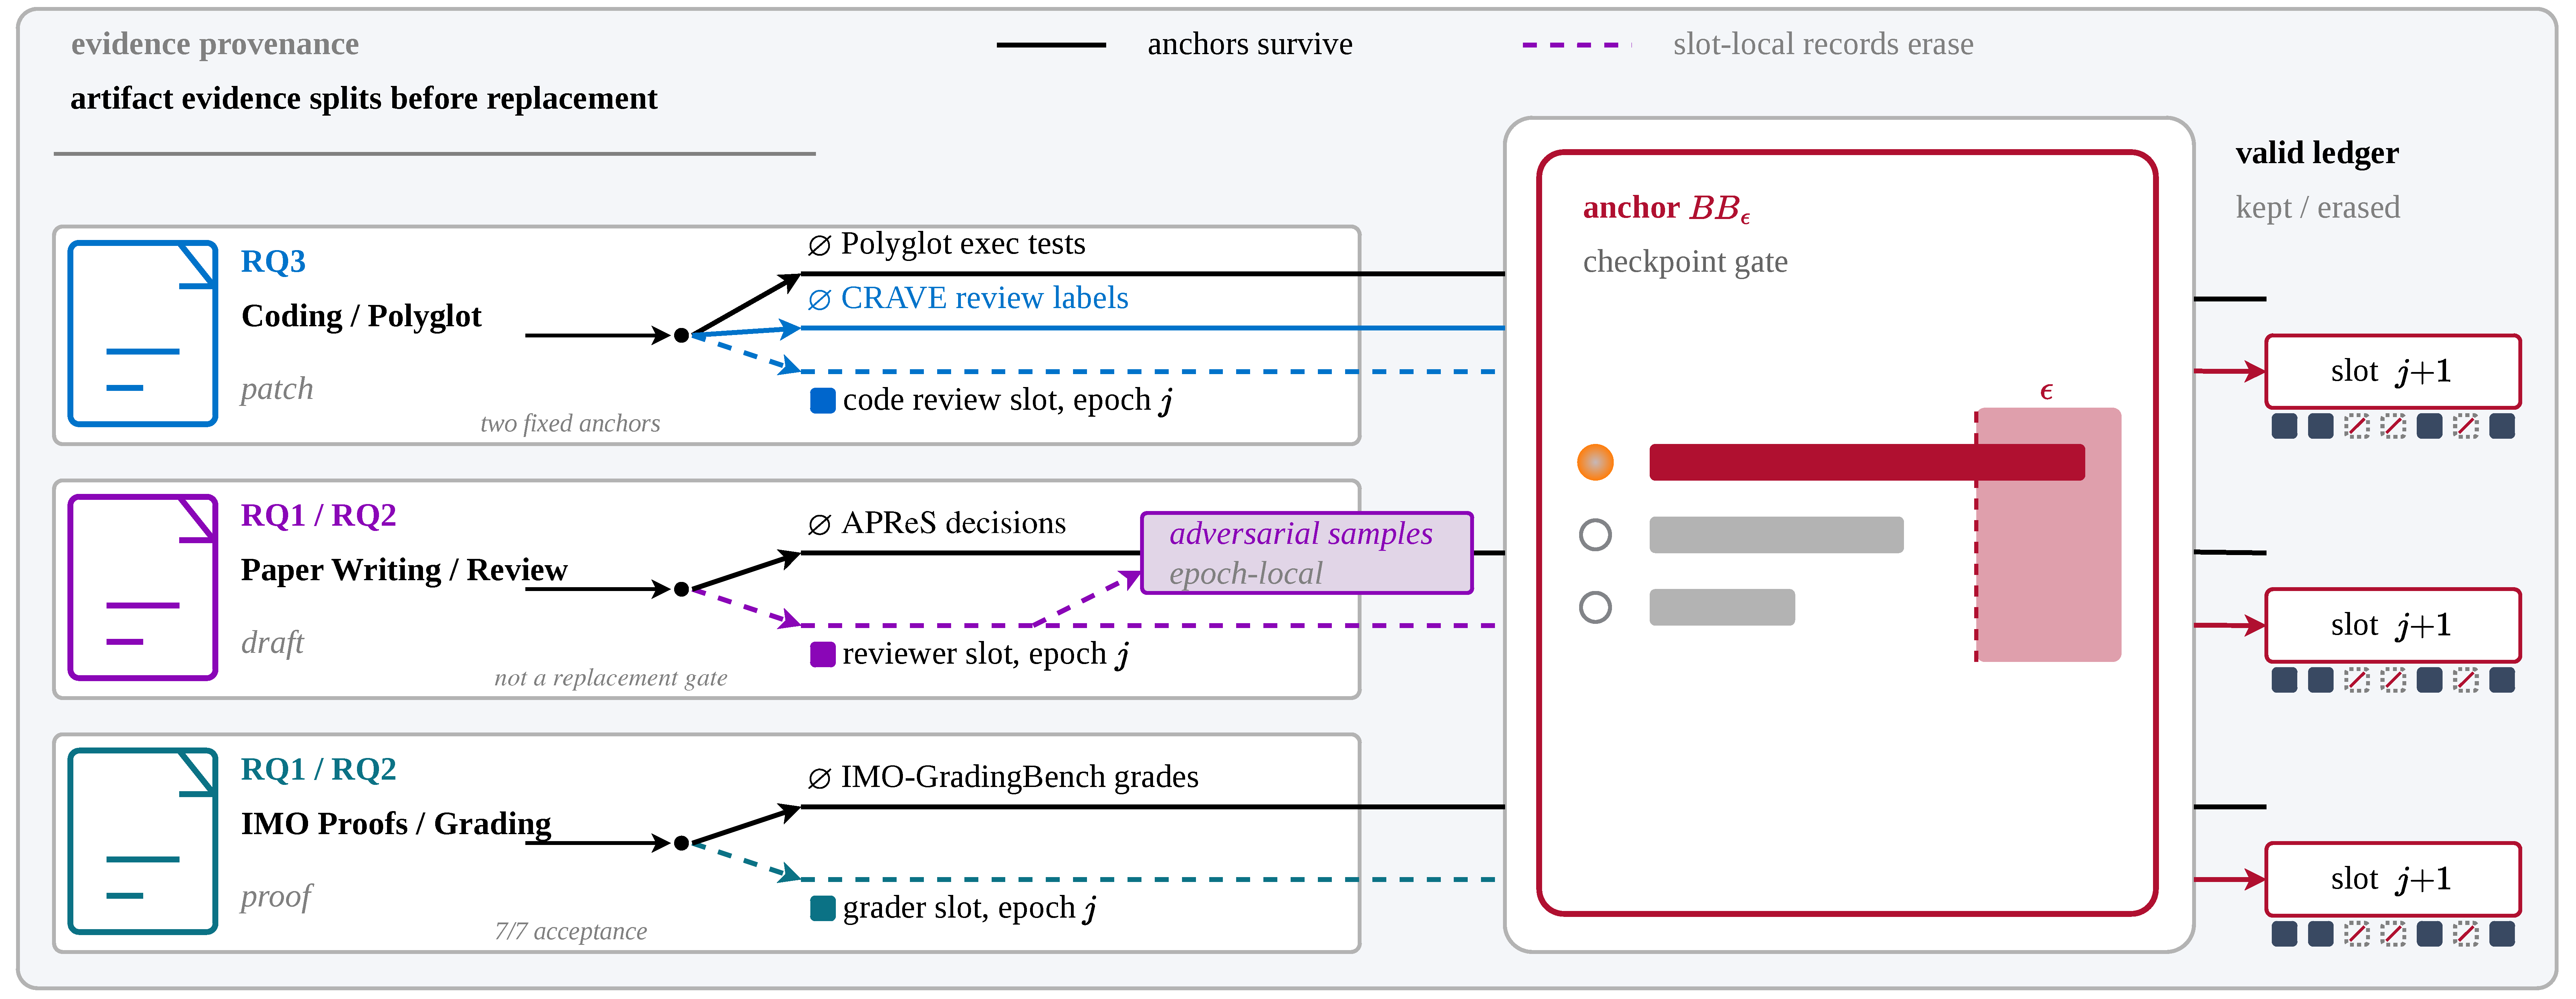
\includegraphics[width=\linewidth]{figures/domain-utilities-diagram-v3-tnr.pdf}
\caption{\textbf{Each domain separates durable anchor evidence from epoch-local evaluator records.} \emph{Left:} fixed ground-truth anchors (solid lines) survive evaluator replacement, while epoch-frozen evaluator-slot records (dashed lines) are local to epoch $j_m$. \emph{Middle:} only evaluator-independent anchor evidence enters the $\epsilon$-best-belief evaluator replacement gate. \emph{Right:} after replacement, anchors remain valid while records from the displaced evaluator slot are erased before epoch $j_m+1$.}
\label{fig:domain-utilities}

\end{widefigure}

\subsection{Models and Run Identities}
\label{app:fm}

Every search run in the main experiments of the paper, held-out evaluation, and panel-scoring call uses \gptlow (low). The cost-reduction ablation of \cref{sec:reducing_search_costs} changes only the search-time task-agent route: the meta-agent remains \gptlow (low), the paper-domain task-agent calls use \nemotronultra during search, and the final endpoint scoring is run with the same \gptlow (low) reviewer as the main paper. \nemotron~\citep{nemotron_super} is used only in the mechanism ablations of \cref{app:nemotron-ablations}. We display the blended token totals: train-time generation and evaluation calls are counted together with search-time utility evaluations~(\cref{sec:method:train}). Overall, there are eight main experiments, one per domain per baseline: coding (\ourmethod{} and \hgmh), paper writing (one \ourmethod{} run yielding the writer, reviewer, and adversarial critic, plus the \hgmh reviewer and the \hgmh writer), and proof (one \ourmethod{} run yielding the prover and grader, plus the \hgmh grader and the \hgmh prover). Every task runs to the same total budget; \hgmh receives the identical exploration budget and typically plateaus earlier. Each agent is read at the point its search reaches its best-belief selection. We allow more powerful models to delegate token processing to cheaper ones. For this paper, we gave \gptlow (low) access to \nemotron; however, we never observed this functionality being used. Similarly, we imposed generous budget caps as a safeguard for expansions and evaluations, which the meta-agent did know about, potentially altering its behavior; however, we never observed an individual node approaching them. Stricter caps may have caused early eval/expansion termination.

\subsection{Search and Scheduling Settings}
\label{app:hyperparams}

Search runs the \hgm clade metaproductivity search of \cref{app:prelim} with frozen evaluator slots and checkpoint-only replacement; replacement and best-belief selection share the $\epsilon$-best-belief rule of \cref{app:swap-rule} applied to nodes with at least $5$ accumulated evaluations. \Cref{tab:settings-fixed} lists the fixed search configuration and \cref{tab:settings-editable} the meta-agent-editable surface with its initial values. Any hyperparameter not listed is taken from \citet{wang2025huxley}. To determine the search budget, we considered the reported $8{,}000$ evaluation budget used by \citet{wang2025huxley} for a single task, chose an economical middle-ground between doubling the search budget for our two task pairs~($16{,}000$) and using the same budget as a single task, settling on $12{,}288 = 8{,}192 + 4{,}096$. 

\begin{table}[ht]
\centering
\caption{\textbf{Fixed search configuration shared by the eight headline runs.} These constants are held fixed across every run and are not exposed to the meta-agent. No search cool-down is used.}
\label{tab:settings-fixed}
\small
\begin{tabular}{@{}ll@{}}
\toprule
Setting & Value \\
\midrule
\multicolumn{2}{@{}l}{\textit{Models and budget}}\\
Base model & \gptlow (low) \\
Ablation model & \nemotron \\
Total budget per run & $12{,}288$ evaluations \\
Train samples per node & $3$ \\
\addlinespace
\multicolumn{2}{@{}l}{\textit{Selection and scheduling}}\\
Best-belief quantile & $\epsilon=0.05$, five-outcome anchor minimum \\
Checkpoint schedule & power-of-two ($\rho=2$) \\
UCB-Air expansion exponent & $\alpha=0.6$ (inherited, \citealp{wang2025huxley}) \\
Expansion gate & expand when $N_t^{\alpha}\geq|\mathcal{T}_t|$ \\
Exploration--exploitation scheduler & $B/b$ ($b$ = remaining budget) \\
\addlinespace
\multicolumn{2}{@{}l}{\textit{Data splits}}\\
Test sets (\apres / \imogradbench / \crave) & $100$ items each \\
\polyglot train split & $10$ items \\
\polyglot validation split & $49$ items \\
\polyglot test split & $166$ items \\
\addlinespace
\multicolumn{2}{@{}l}{\textit{Budget caps}}\\
Expand cap & \$25, $1{,}200$\,s \\
Train cap & \$8, $900$\,s \\
Validation cap & \$25, $1{,}200$\,s \\
\bottomrule
\end{tabular}
\end{table}

\begin{table}[ht]
\centering
\caption{\textbf{Meta-agent-editable surface and its initial values.} Every setting below is exposed to the meta-agent, which may modify it during search.}
\label{tab:settings-editable}
\small
\begin{tabular}{@{}ll@{}}
\toprule
Setting & Initial value \\
\midrule
Output tokens per call & $32{,}768$  \\
Timeout, run & $86{,}400$\,s \\
Timeout, eval & $1{,}200$\,s \\
Timeout, LLM & $300$\,s \\
Timeout, shell & $120$\,s \\
Coder tool calls per task & $\leq 16$ \\
Meta-agent tools & persistent bash ($120$\,s); editor; delegation \\
Meta-agent tool calls per turn & $\leq 40$ \\
\bottomrule
\end{tabular}
\end{table}

\subsection{Held-Out Evaluation Protocols}
\label{app:domain-protocols}

\noindent\textbf{Coding / \polyglot.}~~Generated patches are checked by execution on $166$ held-out tasks. \Cref{tab:raw-counts} carries the counts.

\noindent\textbf{Paper writing / review.}~~Reviewer slots are anchored to \apres conference decisions; the first epoch trains the reviewer on \apres decisions and freezes it as the writer's search-time critic, and replacement itself stays anchored to \apres alone. Reviewer best-belief agents are scored on $100$ held-out \apres papers for accuracy and acceptance~(\cref{tab:raw-counts}); writer best-belief agents are scored on $100$ generated papers per writer by the fixed panel of four reviewers in \cref{tab:paper-writer-cross-reviewer}.

\noindent\textbf{IMO grading / proof writing.}~~Grader slots are anchored to \imogradbench human grades; grader best-belief agents are scored on $100$ held-out items for exact match and normalized mean absolute error. Provers write proofs for $20$ IMO problems each, scored by the fixed panel of three graders, with every per-grader cell in \cref{tab:proof-per-grader}. \texttt{Pass@6} counts proofs scoring at least $6$ of $7$ points; \texttt{Pass@7} requires full credit and is a disclosed trade-off against the static baseline~(\cref{sec:experiments}).

\noindent\textbf{Uncertainty estimation.}~~Uncertainties in the main-text tables pool raw outcomes. For the writer panel~(\cref{tab:paper-writer-cross-reviewer}), each reviewer cell reports the $95\%$ Jeffreys half-width over its $N=100$ paper outcomes, and the Mean column pools all $N=400$ paper $\times$ reviewer outcomes for its own Jeffreys half-width. For the prover panel~(\cref{tab:imo-proof-cross-grader}), each cell pools the $N=60$ raw outcomes ($20$ problems $\times$ $3$ graders): Score ($0$--$7$) is mean $\pm$ s.e.m., and \texttt{Pass@6} / \texttt{Pass@7} are pooled pass rates $\pm$ s.e.m.\ ($\sqrt{\hat p(1-\hat p)/N}$). The writer-panel cells are thus $95\%$ intervals and the prover-panel cells a single standard error (roughly $68\%$ coverage), so their widths are not directly comparable across the two panels.

\noindent\textbf{Cost-reduction ablation.}~~The \nemotronultra ablation~(\cref{sec:reducing_search_costs}) reuses the paper-writing/review protocol of \cref{app:domain-protocols}. The search-time task-agent calls use \nemotronultra, while final \apres reviewer endpoints are scored with \gptlow (low), using the same held-out $N=100$ \apres set. Agent selection uses $\epsilon$-best-belief with $\epsilon=0.05$. Search cost in \cref{fig:nemotron-cost-shift} is reported as \gptlow-price-equivalent blended tokens. We charge expansion to \gptlow and search-time task-agent evaluation calls to \nemotronultra. We use \$$5$/M input and \$$30$/M output tokens for \gptlow~\citep{openai2026pricing}, and \$$0.5$/M input and \$$2.2$/M output tokens for \nemotronultra from \texttt{DeepInfra} pricing~\citep{deepinfra2026pricing}. Similar to the observed cost split of \cref{fig:analysis-cost}, approximately $20\%$ of search cost is expansion and is charged at \gptlow prices, while $80\%$ is repeated task-agent evaluation. The repeated-evaluation calls are input-heavy, so they are accounted for primarily using the conservative input-price ratio $0.5/5=0.10$; the output-price ratio is smaller ($2.2/30=0.073$). Thus a \nemotronultra blended-token total $B$ is converted to roughly $0.20B + 0.80(0.10B)=0.28B$ \gptlow-price-equivalent blended tokens. This gives a $1.87$M \gptlow-price-equivalent cost for the selected \nemotronultra reviewer agent ($B=6.68$M).

\subsection{Initial Agents and Prompts}
\label{app:prompts}

The initial workspace is identical across all experiments; every task agent began as the minimal template below plus a short per-domain output format. The meta-agent instruction states explicitly that utility is computed on a held-out validation set it never sees and that memorized training answers do not transfer to it, so the visible train feedback of \cref{sec:method:train} informs self-modification without being the selection target. The only engineered prompts in the study belong to the control runs: the frozen \sakana reviewer and \proofautograder. Every evaluator behavior reported beyond these formats (checklists, rubric, acceptance standard) was produced by the search~(\cref{app:evaluator-evolution}).

Every task agent is one LLM call from a shared template with no role-specific code.

\begin{promptbox}{Shared task-agent template (all roles)}
\begin{PromptVerb}
You are an agent.

Task input:
```
{inputs}
```

{output_format}
\end{PromptVerb}
\end{promptbox}

The per-domain output formats append a short schema to this template. The paper reviewer is provided below as an example; the writer, IMO grader and prover, and code reviewer differ only in the schema they request, and the coder is the one role with tool access in the initial configuration (bash, editor, and model delegation; the initial workspace allows at most $16$ tool calls per task, a budget the search later raised on both winning chains, \cref{tab:chains-polyglot}). An unparseable output counts as a failure.

\begin{promptbox}{Initial output format: paper reviewer (also scores writer outputs and the adversarial pool)}
\begin{PromptVerb}
You are reviewing the paper above for a top ML venue. Read it carefully
and decide whether to Accept or Reject it.

Respond with one JSON block:
{
  "Summary": "...", "Strengths": [...], "Weaknesses": [...],
  "Decision": "Accept" | "Reject"
}
For "Decision", use only "Accept" or "Reject".
\end{PromptVerb}
\end{promptbox}


The self-modification proposer receives the following instruction verbatim; \texttt{\{repo\_path\}}, \texttt{\{iterations\_left\}}, and \texttt{\{eval\_path\}} are filled by the harness.

\begin{promptbox}{The meta-agent instruction (verbatim, all headline runs)}
\begin{PromptVerb}
Modify any part of the codebase at `{repo_path}` to improve performance
on the active evaluation domains. This includes your OWN code -- the
meta-agent's loop, prompts, tool surface, and the task-agent harness.
Improving your own self-improvement abilities compounds across future
generations and may lead to better outcomes in the long run than only
optimizing the per-domain task agents.

You have {iterations_left} expansions remaining.

Available LLM models for one-shot delegation are listed in
`{repo_path}lineage/MODEL_CATALOG.md`. Use the `query_model` tool to
fire a one-shot call to a different model with
(prompt, id, effort, max_tokens) -- useful for offloading bulk text
generation or sanity-checking your reasoning against a different model.
The call has no chat history and no tools; it's tokens in, tokens out.

Live remaining budget for this expansion is prepended to every chat
turn by the host harness. The host harness/proxy is the only budget
authority; do not infer spend from local transport-library estimates,
token estimates, or model-provider defaults. Read the current remaining
budget before each action, including tool use and one-shot model
delegation, and scale the number and size of calls to fit it.

Prior generation artifacts are at `{eval_path}`. Each ancestor
`gen_<id>/` contains:
  - `<domain>_eval/predictions.csv` -- task-agent outputs paired with
ground-truth labels on the TRAIN split. The only sample-level outcome
data you can see directly.
  - `agent_output/meta_agent_chat_history.md` -- the full transcript of
that predecessor's reasoning. The highest-signal artifact: what was
tried, what worked, what failed. Future generations will read YOUR chat
history, so explain your reasoning clearly.
  - `agent_output/model_patch.diff` -- the code edit the predecessor's
meta-agent produced. Absent on `gen_initial/` (no agent edits there).
  - `metadata.json` -- parent_genid, parent_agent_success, lineage info.

CRITICAL: your utility is computed on a HELD-OUT validation set you
NEVER see. The train predictions you can read are feedback for study
only. Do NOT hardcode answers, memorize specific question ids, or
otherwise overfit to the train samples -- those tricks score perfectly
on train and 0 on validation, which is what actually drives selection.

Outcomes are binary (1=correct, 0=incorrect) and a node's utility is
the mean of its validation outcomes per (role, task). The evaluator is
external -- improving your agents to genuinely produce better outputs
is the path forward; gaming the parser or breaking the harness scores 0.

Each `<domain>_eval/report.json` lists `question_ids_passed` and
`question_ids_failed`. A failed qid means either the LLM's output
couldn't be parsed (counts as outcome=0 by convention) or it parsed but
predicted the wrong answer; both are visible in `predictions.csv`
row-by-row.
\end{PromptVerb}
\end{promptbox}

The meta-agent's runtime constants are in \cref{tab:settings-editable}; each expansion's lease is announced in a live budget header prepended to every turn, and train and validation calls carry their own leases.

\section{Results and Ablations}
\label{app:extended-results}

\subsection{Raw Held-Out Counts}
\label{app:raw-counts}

\begin{table}[H]
\centering
\caption{\textbf{Raw held-out counts at selection} behind \cref{sec:exp-polyglot,sec:exp-writer}.}
\label{tab:raw-counts}
\small
\begin{tabular}{l S[table-format=3.0,round-mode=none] S[table-format=2.0,round-mode=none]}
\toprule
Reviewer & {Accuracy} & {Accept.} \\
\midrule
\hgmh specialist (node 51) & 88 & 45 \\
\ourmethod specialist (node 49) & 84 & 40 \\
\ourmethod generalist, pre-repl.\ (node 78) & 84 & 42 \\
\ourmethod adversarial, post-repl.\ (node 31) & 80 & 32 \\
\dgmh (published) & 73 & 25 \\
\sakana prompt & 63 & 13 \\
\bottomrule
\end{tabular}

\vspace{0.6em}
{\itshape Reviewers: $n=100$ held-out \apres papers.}

\vspace{0.9em}
\begin{tabular}{l S[table-format=3.0,round-mode=none]}
\toprule
Best-belief agent & {Passes} \\
\midrule
\ourmethod specialist (node 104) & 119 \\
\ourmethod generalist (node 100) & 119 \\
\hgmh (node 95) & 116 \\
\bottomrule
\end{tabular}

\vspace{0.6em}
{\itshape Coders: $n=166$ held-out \polyglot tasks, eval-matched protocol.}
\end{table}

\begin{widetable}[H]
\centering
\small
\setlength{\tabcolsep}{3.2pt}
\caption{\textbf{Per-grader proof scores behind \cref{tab:imo-proof-cross-grader}.}}
\label{tab:proof-per-grader}
\begin{tabular}{l *{9}{S[table-format=2.1,round-mode=none]}}
\toprule
& \multicolumn{3}{c}{\proofautograder} & \multicolumn{3}{c}{\hgmh grader (node 45)} & \multicolumn{3}{c}{\ourmethod grader (node 22)} \\
\cmidrule(lr){2-4}\cmidrule(lr){5-7}\cmidrule(lr){8-10}
Prover & {Mean} & {P@6} & {P@7} & {Mean} & {P@6} & {P@7} & {Mean} & {P@6} & {P@7} \\
\midrule
Static \imocode prover & 4.05 & 55.0 & 55.0 & 4.10 & 55.0 & 55.0 & 4.05 & 55.0 & 55.0 \\
\hgmh prover & 3.55 & 50.0 & 45.0 & 3.65 & 50.0 & 45.0 & 4.00 & 55.0 & 45.0 \\
\ourmethod prover (generalist) & 3.55 & 50.0 & 45.0 & 3.70 & 50.0 & 45.0 & 3.95 & 55.0 & 45.0 \\
\bfseries \ourmethod prover (specialist) & \bfseries 3.85 & \bfseries 55.0 & \bfseries 40.0 & \bfseries 4.20 & \bfseries 60.0 & \bfseries 45.0 & \bfseries 4.95 & \bfseries 70.0 & \bfseries 60.0 \\
\bottomrule
\end{tabular}
\end{widetable}
\FloatBarrier
\subsection{Mechanism Ablations}
\label{app:nemotron-ablations}

Below, we provide ablations that isolate components of controlled utility evolution, replacement, the adversarial pool, and selective erasure, each turned off in a paper-review run~(\cref{tab:nemotron-runs}). Every mechanism and hyperparameter is held fixed; only the underlying model changes, to \nemotron. Compared to the \gptlow runs, the smaller context window of \nemotron triggers frequent compaction. Furthermore, its replacement decisions partly reflect reliability fixes rather than review logic~(\cref{app:analyses:patches}). 

\noindent\textbf{The fixed critic saturates.}~~With replacement off the writer ends at $75/75$ accepted validation papers, trivially raising acceptance by the frozen critic past the human acceptance rate. 

\noindent\textbf{Replacement alone (adversarial pool off) escapes that plateau.}~~Ending at an anchor result of $52/57$; the writer re-bases after each replacement instead of saturating a moving judge, so replacement suffices for progress while the adversarial pool shapes \emph{which} reviewer is selected~(\cref{sec:exp-adversarial}). 

\noindent\textbf{Without erasure the utility stays stale.}~~Retired-critic rows remain in the official utility; the slot oscillates through an A$\to$B$\to$A return of a displaced critic; evaluator replacements stop triggering as stale evidence accumulates, driving the search to explore the same nodes repeatedly.

\noindent\textbf{Adversarial pool matches replacement-only at search time.}~~The adversarial pool primarily serves to better delineate the decision boundary between human- and \AI-generated text, thus it primarily impacts downstream reviewer evaluations on writer-generated text.

\begin{widetable}[H]
\centering
\caption{\textbf{Mechanism ablations on the evaluator-independent anchor.} All runs use a $12{,}288$-evaluation budget. Reviewer anchor accuracy is comparable across runs, while writer acceptance ($\dagger$), scored by each run's own critic, is not. Cells report mean $\pm$ 95\% Jeffreys interval.}
\label{tab:nemotron-runs}
\small
\setlength{\tabcolsep}{4.5pt}
\begin{tabular}{l c c c c c}
\toprule
Run & Repl. & Pool & Erase & Writer val.\ acc.\ (\%)$^{\dagger}$ & Reviewer anchor acc.\ (\%) \\
\midrule
Full mechanism & on & on & on & $90.1$\,{\color{black!55}\scriptsize$\pm 3.5$} & $95.0$\,{\color{black!55}\scriptsize$\pm 10.3$} \\
Replacement only & on & off & on & $89.5$\,{\color{black!55}\scriptsize$\pm 13.7$} & $91.2$\,{\color{black!55}\scriptsize$\pm 7.4$} \\
No erasure & on & on & off & $90.0$\,{\color{black!55}\scriptsize$\pm 10.7$} & $92.9$\,{\color{black!55}\scriptsize$\pm 10.8$} \\
\addlinespace
Fixed critic & off & off & {--} & $100.0$\,{\color{black!55}\scriptsize$\pm 1.7$} & $78.2$\,{\color{black!55}\scriptsize$\pm 4.4$} \\
\bottomrule
\end{tabular}
\end{widetable}

\subsection{Where Cost and Progress Come From}
\label{app:analyses}

We now present how the actual search process evolved in terms of compute allocation and edits.

\subsubsection{Cost decomposition}
\label{app:analyses:budget}

Every model call is related to workspace expansion, train-time evaluation, or validation evaluation. The overall run cost is dominated by validation: across the three main-experiment runs, validation carries roughly $65$--$69\%$ of blended tokens, expansion $18$--$23\%$, and train-time evaluation (at three train samples per node) $12$--$14\%$~(\cref{fig:analysis-cost}). Allocating more train samples to each meta-agent may allow for more efficient search due to more context, thus its possible that the current share of tokens going to train-time evaluation is too low.

\begin{figure}[H]
\centering

\includegraphics[width=\linewidth]{figures/fig_analysis_cost.pdf}
\caption{\textbf{Blended-token cost decomposition of the three headline \gptlow (low) runs} into workspace expansion, train-time evaluation, and validation evaluation.}
\label{fig:analysis-cost}
\end{figure}


\subsubsection{Patch surfaces}
\label{app:analyses:patches}

We classify every lineage edge's patch by the code surface it modifies. Shared surfaces, the task-agent code and infrastructure used by more than one role, carry $59$--$90\%$ of accepted patches in every \gptlow run~(\cref{fig:analysis-transfer}). For example, the \polyglot run concentrates its improvements on shared and infrastructure surfaces that generalize across roles. We posit this is because the meta-agent realizes that role-specific patches each drive a single utility and generalize less. The \nemotron run is the outlier as it heavily targets the meta-agent's instruction module ($42\%$ of edges), potentially to improve its reliability.

\begin{figure}[H]
\centering

\includegraphics[width=\linewidth]{figures/fig_analysis_transfer.pdf}
\caption{\textbf{Patch surfaces by run}, classifying each accepted lineage edge by the code surface it modifies (task-agent shared, infrastructure, role-specific, meta-agent module, or notes).}
\label{fig:analysis-transfer}
\end{figure}



\section{What the Co-Evolution Discovered}
\label{app:evaluator-evolution}

Every evaluator role is a prompt entry in one shared workspace file, so each evaluator's behavioral history reads directly from its lineage. The initial role prompts are minimal~(\cref{app:prompts}); across every role, the search's most common move rewrites a vague one-line instruction into a specific, criterion-bearing rubric, and the rules it produced are quoted below. Because the starting prompts are minimal, a stronger initial prompt would raise every method's scores together without changing the co-evolution comparison, which holds each method to the same starting point.

\subsection{What the Evolved Evaluators Changed}
\label{app:evaluator-evolution:reviewer}

The adversarial reviewer's lineage rewrites the one-line initial instruction once into a conjunctive acceptance standard, while the pre-replacement generalist carries a two-sided calibration.

\begin{promptbox}{Evolved rule: the adversarial reviewer's conjunctive standard (gen\,4)}
\begin{PromptVerb}
... Use a realistic selective-conference standard: accept only if the
paper has a clear nontrivial contribution, technically sound
methodology/theory or experiments, adequate positioning against prior
work, and claims supported by evidence; reject papers with missing
validation, unclear novelty, serious technical gaps, or overclaiming.
Do not be swayed by fluent writing alone.
\end{PromptVerb}
\end{promptbox}

\begin{promptbox}{Evolved rule: the displaced generalist's two-sided calibration}
\begin{PromptVerb}
... Calibrate the decision holistically rather than requiring
perfection: a paper with a coherent contribution and adequate evidence
should be accepted despite presentation flaws, while impressive writing
without substantiated experiments or technical substance should be
rejected.
\end{PromptVerb}
\end{promptbox}

Both wordings appeared early in their lineages; the adversarial pool changed which lineage was selected to reject a greater fraction of \AI-generated papers.

\subsection{The Co-Evolved Grader}
\label{app:evaluator-evolution:grader}

The grader reached its reported form in exactly two patches, both quoted here; the initial instruction assigns one of four labels with no rubric. The first patch introduces the persona, the two-step milestone procedure, the points mapping, and a strictness rule, and the same patch introduces the prover prompt, so the prover and grader entered the workspace together. A later patch removes the blanket strictness while keeping the milestone procedure and points mapping.

\begin{promptbox}{Evolved rule: the grader's first rewrite (gen\,2)}
\begin{PromptVerb}
You are an expert, conservative IMO proof grader. ... First identify
the key required steps from the guidelines; then check whether the
student's text actually proves them rigorously, ignoring unsupported
claims, handwaving, and statements merely resembling the reference.

Use this mapping unless the problem-specific guidelines say otherwise:
- correct: a complete rigorous solution (7/7).
- almost: essentially complete with only a minor local gap or
  arithmetic slip (6/7); do NOT use for missing major lemmas.
- partial: substantial guideline-listed progress, but not a
  near-complete proof (1/7).
- incorrect: no substantial credited progress or a fundamentally
  flawed argument (0/7).

Be especially strict with advanced geometry/combinatorics solutions
that invoke large unproved lemmas ...
\end{PromptVerb}
\end{promptbox}

\begin{promptbox}{Evolved rule: the co-evolved grader's recalibration (gen\,22)}
\begin{PromptVerb}
Calibrate generously but not naively: do not require the student's
proof to match the reference solution, and do not downgrade merely
because a standard theorem/lemma is cited tersely, the exposition is
compressed, or a repairable statement is slightly misphrased. ...
Downgrade to partial/incorrect only for a genuinely fatal gap, a false
central claim with no reasonable repair, or failure to prove a
guideline milestone.
\end{PromptVerb}
\end{promptbox}

Its behavior in the cross-grader panel of \cref{tab:imo-proof-cross-grader} follows from these patches.

\subsection{The \polyglot Code Reviewer}
\label{app:evaluator-evolution:critic}

The code-review slot was replaced three times; the initial instruction asks for a pass/fail verdict on general code quality, and the three incumbents' rules are quoted below. The third branches from an earlier ancestor than the second, so it does not inherit the second's bullets. Across the three replacements, the slot moves toward evidence-bounded review: each incumbent narrows what counts as a failure to defects in the diff itself.

\begin{promptbox}{Evolved rules: the three promoted code reviewers}
\begin{PromptVerb}
Node 19 (gen 5): You are a pragmatic senior maintainer reviewing a
proposed patch. ...
- PASS when the patch plausibly fixes/adds the intended behavior, is
  localized, and has no clear correctness, compilation, security, or
  data-loss defect. ...
- FAIL only for a concrete blocker: obvious wrong behavior, broken API
  usage, compile/type errors visible in the diff, missing essential
  cases, flaky/meaningless tests, ...
- ... If evidence is balanced, prefer pass.

Node 34 (gen 34, appends): - Review in this order: (1) infer the
intended user-visible behavior ..., (2) check whether production code
implements it, (3) look for definite regressions or syntax/type
errors, (4) only then consider style, test coverage, and
maintainability. Style concerns without a concrete correctness risk
should not cause fail. ... FAIL only when you can point to a specific
scenario that remains broken ...

Node 86 (gen 59, extends the blocker rule): ... Do not invent blockers
from missing project context; the diff alone must show the defect.
- PASS broad but coherent mechanical migrations, CI/build-artifact
  pipeline updates, ... and test-only fixes when they are internally
  consistent ...
- For security/credential-looking files, fail only for an actual
  exposed secret or dangerous permission; ...
\end{PromptVerb}
\end{promptbox}

\subsection{Winning Lineages}
\label{app:lineages}

\begin{widefigure}[t]
    \centering
    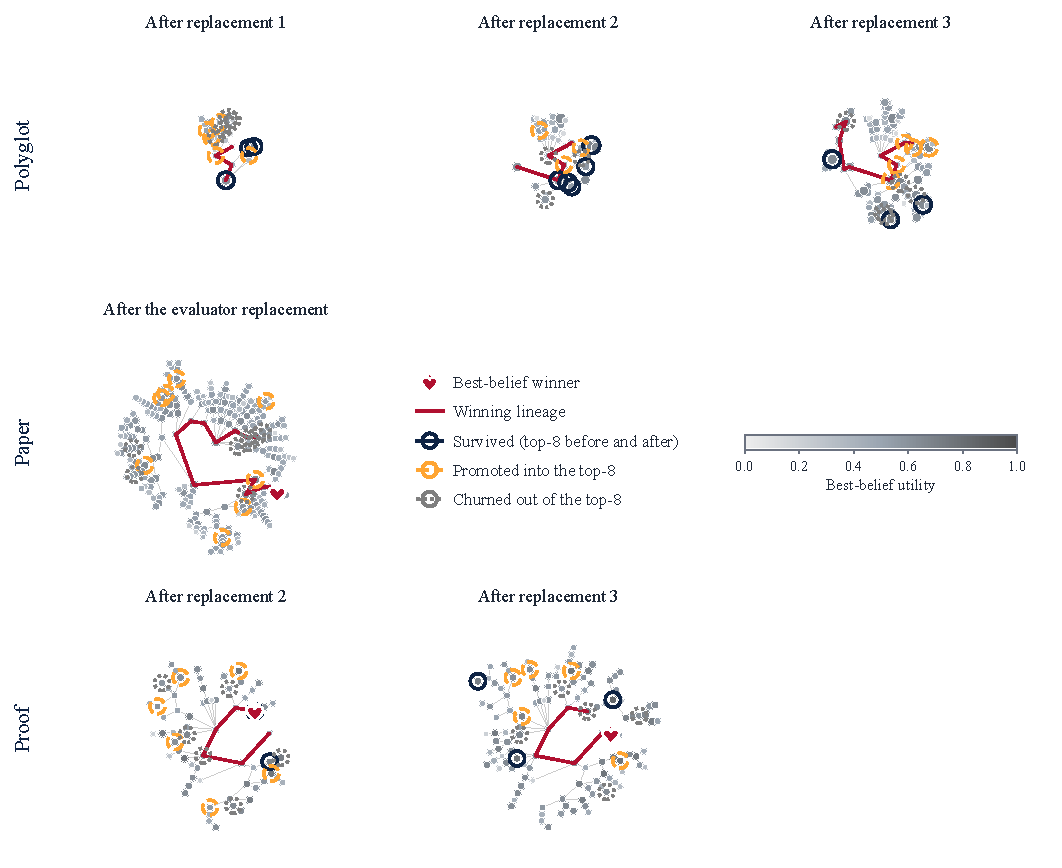
\includegraphics[width=\linewidth]{figures/fig_tree_utilities.pdf}
    \caption{\textbf{What each evaluator replacement keeps versus what it re-ranks, in all three headline domains.} Rows are domains (top to bottom: \polyglot, paper, proof); columns are that run's shown evaluator replacements, each drawing the archive as it stood at that replacement (radial layout, node color is best-belief utility and size is evidence count). Among the top-$8$ leaderboard nodes at each replacement, navy rings survived the re-ranking, amber rings are lineages the new criterion promotes into the top-$8$, and gray rings are churned out. Replacements with fewer than $20$ ranked nodes are omitted, as in \cref{fig:transition-rerank}, so the proof run's first replacement is not shown.}
    \label{fig:lineage-trees}
\end{widefigure}

We now show full lineages across our runs. Each archive node stores its parent, its cumulative self-modification as a unified diff, and the meta-agent transcript that produced it; \cref{fig:lineage-trees} draws the three archives, \cref{tab:chains-polyglot,tab:chains-paper,tab:chains-proof} list every step, and quoted phrases are from the meta-agents' own summaries. The generalist chain's largest gain is not a prompt change but a code repair, and the same node was later promoted into the code-review slot at the first checkpoint. The adversarial reviewer's standard arrived before any replacement; the adversarial pool selected that lineage at the second epoch~(\cref{app:evaluator-evolution}). 

\begin{widetable}[t]
\centering
\caption{\textbf{\polyglot winning chains; both final best-belief agents score $119/166$ held out.}}
\label{tab:chains-polyglot}
\small
\begin{tabular}{@{}r >{\raggedright\arraybackslash}p{0.84\linewidth}@{}}
\toprule
{Node} & Modification \\
\midrule
\multicolumn{2}{@{}l}{\textit{specialist} (final $119/166$)}\\
4 & coder tool budget $16{\to}40$; review calibration; catalog-path fix \\
35 & coder workflow: one tool call at a time, prefer exact algorithms \\
51 & review balance against blindly passing bad patches \\
104 & parse retry; label normalization; concrete-blocker review rule \\
\midrule
\multicolumn{2}{@{}l}{\textit{generalist} (final $119/166$)}\\
5 & parse retry; tool budget $16{\to}24$; concrete-blocker review \\
19 & untracked-artifact and symlink diff hygiene \\
33 & the same hygiene applied to a second code path \\
42 & one tool call per turn; preserve existing public APIs \\
72 & read problem text and tests first; wider artifact filter \\
78 & final-output reminder; conservative label normalization \\
93 & dedicated artifact-review format; pass plausible localized fixes \\
100 & JSON-serialized tool results (transcript-corruption fix) \\
\bottomrule
\end{tabular}
\end{widetable}

\begin{widetable}[t]
\centering
\caption{\textbf{Paper-domain winning chains.} The writer chain passes through the reported reviewer (49) and generalist (78); the adversarial reviewer (31) descends separately.}
\label{tab:chains-paper}
\small
\begin{tabular}{@{}r >{\raggedright\arraybackslash}p{0.84\linewidth}@{}}
\toprule
{Node} & Modification \\
\midrule
\multicolumn{2}{@{}l}{\textit{writer}}\\
7 & stronger authoring prompt; runtime prompt nudges \\
11 & parse-repair retry; $8{,}192$-token writer output cap \\
17 & present raw paper text instead of the input dictionary \\
37 & remove global LLM monkeypatch \\
49 & writer returns raw text, not JSON-wrapped continuations \\
78 & two-sided review calibration; no acceptance-seeking prose \\
81 & format hygiene in the client; revert import hook that could hang \\
89 & continue from the exact stopping point; longer word target \\
150 & liberal unwrapping of writer output (recovers wrapped papers) \\
154 & \textbf{area-chair review standard}; bounded-evidence writing rules \\
\midrule
\multicolumn{2}{@{}l}{\textit{adversarial}}\\
4 & conjunctive selective-conference review standard \\
25 & writer-side review treated as a viability gate \\
31 & self-contained revised paper; $4{,}096$-token output cap \\
\bottomrule
\end{tabular}
\end{widetable}

\begin{widetable}[t]
\centering
\caption{\textbf{Proof-domain winning chains.} The grader's calibration reversal at node 22 is the largest single-step utility gain in any winning chain.}
\label{tab:chains-proof}
\small
\begin{tabular}{@{}r >{\raggedright\arraybackslash}p{0.84\linewidth}@{}}
\toprule
{Node} & Modification \\
\midrule
\multicolumn{2}{@{}l}{\textit{grader}}\\
2 & conservative rubric-aware grading; first prover prompt \\
22 & calibration reversal: do not downgrade terse or compressed proofs \\
\midrule
\multicolumn{2}{@{}l}{\textit{prover}}\\
3 & parse retry; lemma-justification and case-coverage prompt \\
11 & partial-versus-incorrect distinction; hidden-assumption checks \\
19 & second-pass self-revision with an adversarial checker \\
66 & disable the inherited self-revision (rollout below) \\
\bottomrule
\end{tabular}
\end{widetable}

Two modifications outside the evaluator prompts were the most consequential. The first is node 19's diff-hygiene repair~(\cref{lst:diff-hygiene}); the artifact filter is the load-bearing line, quoted from its patch.

\begin{lstlisting}[style=rsdiff, caption={Node 19's diff-hygiene repair (\polyglot run): untracked dependency artifacts and unsafe symlinks are filtered out of submitted patches.}, label={lst:diff-hygiene}]
diff --git a/utils/git_utils.py b/utils/git_utils.py
@@ def diff_versus_commit(git_dname, commit):
     dependency_artifact_roots = {
         "node_modules", ".npm", ".yarn", ".pnpm-store",
         "target", "build", "dist", "__pycache__", ".pytest_cache",
     }
     def should_include_untracked(relpath):
         parts = relpath.split(os.sep)
         if parts and parts[0] in dependency_artifact_roots:
             return False         # skip incidental install artifacts
         file_path = os.path.abspath(os.path.join(git_dname, relpath))
         if os.path.islink(file_path):
             target = os.path.realpath(file_path)
             # drop symlinks resolving outside the checkout
             if not target.startswith(os.path.abspath(git_dname)):
                 return False
         return True
\end{lstlisting}

The second is the prover's three-line retraction of its ancestor's self-revision feature (node 66, \cref{lst:prover-retraction}).

\begin{lstlisting}[style=rsdiff, caption={Node 66's retraction (proof run): the inherited self-revision pass is disabled by default and the revision instruction is rewritten to preserve sound drafts, on the recorded grounds that revision ``could degrade a correct/near-correct detailed proof into a weaker black-box citation-based proof.''}, label={lst:prover-retraction}]
diff --git a/task_agent.py b/task_agent.py
@@ class TaskAgent(AgentSystem):
-    IMO_PROOF_REVISION_ENABLED = os.environ.get("HYPERAGENTS_IMO_PROOF_REVISION", "1") != "0"
+    IMO_PROOF_REVISION_ENABLED = os.environ.get("HYPERAGENTS_IMO_PROOF_REVISION", "0") == "1"
@@ Draft proof:
-Find any hidden gaps ... If the draft is sound, keep it but make it cleaner.
+Preserve the draft if it is essentially sound; do not replace a detailed proof
+with a shorter answer that relies on an unproved obscure named theorem.
\end{lstlisting}


\section{Theory}
\label{app:proofs}


\subsection{Setting: the \texorpdfstring{\hgm}{HGM} Search Algorithm}
\label{app:prelim}

\ourmethod builds on the Huxley-G\"odel Machine (\hgm)~\citep{wang2025huxley}, which formalizes self-improvement as tree search guided by clade metaproductivity (\cmp), and \hyperagents~(\dgmh)~\citep{zhang2026hyperagents}, which introduces metacognitive self-modification in editable agent workspaces; we review only the assumptions and theory this paper needs, then state the local operating conditions the proofs use.

\subsubsection{Self-Improvement as Tree Search}
\label{sec:prelim:tree}

Following \citet{wang2025huxley}, an archive $\mathcal{T}_t$ of agents forms a tree initialized at $\mathcal{T}_0=\{a_0\}$. At each iteration, the policy either modifies an existing agent or evaluates one:
\[
\begin{gathered}
\mathcal{A}_t = \mathcal{M}_t \cup \mathcal{V}_t,\\
\mathcal{M}_t = \{m_a : a \in \mathcal{T}_t\},
\qquad
\mathcal{V}_t = \{v_a : a \in \mathcal{T}_t\}.
\end{gathered}
\]
A modification action $m_a$ produces a child of $a$; an evaluation action $v_a$ tests $a$ on one task and returns a binary outcome $o\in\{0,1\}$. After a fixed external budget $B$, the system returns the highest-scoring agent in the archive:
\[
a_{\mathrm{final}}
=
\argmax_{a\in\mathcal{T}_B}\operatorname{Score}_\pi(a).
\]
The utility $U(a)$ is the expected binary success rate of agent $a$ under the evaluation protocol. \ourmethod preserves this flat \hgm search algorithm while generalizing what a node contains and how its binary outcomes are produced.

\subsubsection{\texorpdfstring{\hgm}{HGM}-Compatible Operating Conditions}
\label{sec:prelim:assumptions}

These are the local conditions the appendix results need.

\begin{assumption}[\hgm-compatible fixed-criterion search]
\label{assumption:hgm}
For the theoretical analysis of a fixed-criterion self-improvement epoch, assume:
\begin{enumerate}[leftmargin=*,itemsep=0.2em,label=\textbf{C\arabic*.},ref=C\arabic*]
    \item \label{cond:final} The objective is evaluated through the agent selected from the archive after the search budget is spent; intermediate observations guide search but are not separate rewards.
    \item \label{cond:stationary} For any fixed node--task pair under the active criterion, repeated evaluations produce time-homogeneous binary outcomes.
    \item \label{cond:proofs} Any oracle or proof object used by the ideal \hgm theorem is outside the empirical search-evaluation budget.
    \item \label{cond:budget} The empirical scheduler accounts for expansion and evaluation through the externally fixed budget units used by the run.
\end{enumerate}
\end{assumption}

The key condition for \ourmethod is stationarity: \hgm assumes a fixed evaluator, so an early outcome means the same as a late one. \ourmethod preserves the property locally: \cref{sec:method:generative} freezes learned evaluators within an epoch, and \cref{sec:method:utility} permits changes only at checkpoints, followed by selective erasure of records whose meaning depended on the displaced evaluator.

\subsubsection{Clade-Level Metaproductivity}
\label{sec:prelim:cmp}

\citet{wang2025huxley} show that a node's immediate benchmark performance may not predict long-run self-improvement value: a weak node may produce strong descendants. \hgm replaces the G\"odel Machine's intractable proof search over future modifications with archive search over observed descendant productivity, scoring a node on its \emph{clade}, the subtree $C(\mathcal{T},a)$ of $a$ and its descendants, written $C(a)$ when the tree is clear.

\begin{theorem}[\citet{wang2025huxley}]
\label{thm:cmp}
Under \cref{assumption:hgm}, access to the \cmp oracle is sufficient to implement the G\"odel Machine.
\end{theorem}

In practice, \hgm estimates clade-level metaproductivity by pooling binary outcomes over the clade:
\[
\begin{gathered}
\widehat{\cmp}(a)=\frac{n_{\mathrm{success}}^C(a)}{n_{\mathrm{success}}^C(a)+n_{\mathrm{failure}}^C(a)},\\
n_{\mathrm{success}}^C(a)=\textstyle\sum_{a'\in C(a)} n_{\mathrm{success}}(a'),\\
n_{\mathrm{failure}}^C(a)=\textstyle\sum_{a'\in C(a)} n_{\mathrm{failure}}(a').
\end{gathered}
\]
Thompson sampling over the clade-level success and failure counts trades exploration against exploitation, and the UCB-Air gate~\citep{NIPS200849ae49a2} controls tree growth. \ourmethod inherits these mechanisms unchanged; the property the proofs rely on is that the scheduler consumes a flat stream of binary outcomes per node, aggregated over the node's clade. The node representation is the metacognitive workspace of \hyperagents~\citep{zhang2026hyperagents}: each archive node is a shared workspace $w_a$ with $K$ role agents plus a meta-agent that can edit the node's code and coordination, while \hgm search decides which lineage receives expansion and evaluation budget~(\cref{app:fm}).

\subsection{One Rule for Replacement and Selection}
\label{app:controlled_utility_details}

Evaluator slots are frozen within an epoch, challengers are selected by $\epsilon$-best-belief score on anchor evidence, and the promoted evaluator is frozen for the next epoch~(\cref{sec:method:utility}).

\subsubsection{Evaluator replacement rule}
\label{app:swap-rule}

At checkpoint $c$, fix an evaluator slot $m$. Let $e_m^{(j_m)}$ be the incumbent frozen evaluator and let $\mathcal C_m(c)$ be the challenger evaluators with the required evaluator-independent anchor evidence on $\mathrm{GT}_m$. Define
\[
\mathcal E_m(c)
=
\{e_m^{(j_m)}\}\cup\mathcal C_m(c).
\]
For each candidate $e\in\mathcal E_m(c)$, let $S^{\mathrm{gt}}_e$ and $F^{\mathrm{gt}}_e$ be its successes/failures on the anchor. Compute
\[
BB_\epsilon(e)
=
I^{-1}_{\epsilon}\!\left(1+S^{\mathrm{gt}}_e,\,1+F^{\mathrm{gt}}_e\right),
\]
the same $\epsilon$-best-belief score used for final agent selection~(\cref{sec:method:prelim}). Because $BB_\epsilon(e)$ is the $\epsilon$-quantile of the candidate's Beta posterior over anchor outcomes, it is a conservative estimate of the candidate's true accuracy that the candidate exceeds with probability $1-\epsilon$. The selected evaluator is
\[
e_m^\star
\in
\argmax_{e\in\mathcal E_m(c)} BB_\epsilon(e),
\]
with ties favoring the incumbent; if $e_m^\star=e_m^{(j_m)}$, no transition occurs.


\subsection{Working-Posterior Consistency}
\label{app:proofs:role_task_balance}
Fix an epoch vector \(\boldsymbol{j}\) and a node \(a\). Let
\[
\mathcal C_{\boldsymbol{j}}(a)
=
\{(r,d): r\in \mathcal{R}_{\mathrm{elig}}(a,\boldsymbol{j}),\ d\in \mathcal{D}_{r,\mathrm{elig}}(a,\boldsymbol{j})\}
\]
denote the finite set of eligible role--task cells for node \(a\) during epoch \(\boldsymbol{j}\).
For a cell \(c=(r,d)\in \mathcal C_{\boldsymbol{j}}(a)\), let \(p_{c,\boldsymbol{j}}(a)\) be the fixed success
probability of one search evaluation of node \(a\) on role \(r\) and task \(d\)
under the active evaluation criteria of epoch \(\boldsymbol{j}\). The default role/task-balanced target assigns
\[
w_{r,d}
=
\frac{1}{|\mathcal{R}_{\mathrm{elig}}(a,\boldsymbol{j})|}\cdot
\frac{1}{|\mathcal{D}_{r,\mathrm{elig}}(a,\boldsymbol{j})|},
\]
with the obvious renormalization for a smaller eligible set. Generally,
let \(w_c\ge 0\) be weights satisfying
\[
\sum_{c\in \mathcal C_{\boldsymbol{j}}(a)} w_c = 1,
\]
with \(w_c\ge 0\)~(see \cref{prop:validity}).
The corresponding epoch-local role--task balanced utility is
\[
U_{\boldsymbol{j}}(a)
=
\sum_{c\in \mathcal C_{\boldsymbol{j}}(a)} w_c\,p_{c,\boldsymbol{j}}(a).
\]

\begin{proposition}[Consistency of the \hgm working posterior under balanced role--task sampling]
\label{prop:balanced-working-posterior}
Fix an epoch vector \(\boldsymbol{j}\), a node \(a\), and the eligible role--task cell set
\(\mathcal C_{\boldsymbol{j}}(a)\). Consider the subsequence of search evaluations in which
node \(a\) is selected during this epoch. After \(n\) such evaluations, let
\(n_c(n)\) be the number of evaluations assigned to cell \(c\), and let
\[
S_a(n)=\sum_{t=1}^{n} O_t
\]
be the total number of binary successes recorded for node \(a\).

Assume the within-node scheduler is \(w\)-balanced, that is:
\[
\frac{n_c(n)}{n}\longrightarrow w_c
\qquad\text{for every } c\in \mathcal C_{\boldsymbol{j}}(a).
\]
Assume also that, for each cell \(c\), repeated evaluations of \(a\) on \(c\)
satisfy a cell-wise strong law:
\[
\frac{1}{m}\sum_{i=1}^{m} O_{c,i}
\longrightarrow
p_{c,\boldsymbol{j}}(a)
\qquad\text{a.s. as }m\to\infty,
\]
where \(O_{c,i}\) is the \(i\)-th outcome observed from cell \(c\). This condition
holds, for example, when cell-level outcomes are independent Bernoulli trials
with fixed success probability \(p_{c,\boldsymbol{j}}(a)\), or under any stationary
martingale-difference model satisfying the strong law.

Define the \hgm-compatible working posterior
\[
Q_n(a)
=
\operatorname{Beta}\bigl(1+S_a(n),\,1+n-S_a(n)\bigr).
\]
Its mean is
\[
M_n(a)
=
\frac{1+S_a(n)}{2+n}.
\]
Then
\[
M_n(a)
\longrightarrow
U_{\boldsymbol{j}}(a)
=
\sum_{c\in \mathcal C_{\boldsymbol{j}}(a)} w_c\,p_{c,\boldsymbol{j}}(a)
\qquad\text{a.s.}
\]

Thus the pooled Beta accumulator preserves the correct role--task balanced
posterior mean target asymptotically. \(Q_n(a)\) is a working posterior used to retain the flat \hgm success/failure interface for Thompson sampling.
\end{proposition}

\begin{proof}
Fix the epoch vector \(\boldsymbol{j}\), node \(a\), and eligible cell set
\(\mathcal C_{\boldsymbol{j}}(a)\). Write \(p_c\) for \(p_{c,\boldsymbol{j}}(a)\).
Let \(n_c(n)\) be the number of times cell \(c\) is evaluated among the first
\(n\) search evaluations of node \(a\) in this epoch. Let
\[
\widehat p_{c,n}
=
\frac{1}{n_c(n)}
\sum_{i=1}^{n_c(n)} O_{c,i}
\]
whenever \(n_c(n)>0\). Cells with \(w_c=0\) contribute a vanishing fraction of evaluations and drop from the limit, so the cell-wise strong law is applied only on the support \(\{c:w_c>0\}\). For each such cell, \(w_c>0\) and \(n_c(n)/n\to w_c\) give \(n_c(n)\to\infty\), and therefore, by the assumed cell-wise strong law,
\[
\widehat p_{c,n}
\longrightarrow
p_c
\qquad\text{a.s.}
\]

The pooled empirical success rate decomposes by cells:
\[
\frac{S_a(n)}{n}
=
\sum_{c\in \mathcal C_{\boldsymbol{j}}(a)}
\frac{n_c(n)}{n}\,
\widehat p_{c,n}.
\]
Taking limits and using the finiteness of \(\mathcal C_{\boldsymbol{j}}(a)\),
\[
\frac{S_a(n)}{n}
\longrightarrow
\sum_{c\in \mathcal C_{\boldsymbol{j}}(a)}
w_c p_c
=
U_{\boldsymbol{j}}(a)
\qquad\text{a.s.}
\]

The \hgm working posterior is
\[
Q_n(a)
=
\operatorname{Beta}\bigl(1+S_a(n),\,1+n-S_a(n)\bigr),
\]
with mean
\[
M_n(a)
=
\frac{1+S_a(n)}{2+n}.
\]
Moreover,
\[
\left|
\frac{1+S_a(n)}{2+n}
-
\frac{S_a(n)}{n}
\right|
=
\left|
\frac{n-2S_a(n)}{n(n+2)}
\right|
\le
\frac{1}{n+2}.
\]
Hence
\[
M_n(a)-\frac{S_a(n)}{n}\longrightarrow 0,
\]
and therefore
\[
M_n(a)
\longrightarrow
U_{\boldsymbol{j}}(a)
\qquad\text{a.s.}
\]

On the posterior interpretation: the cell-stratified likelihood
\(\prod_{c\in\mathcal C_{\boldsymbol{j}}(a)} p_c^{S_c(n)}(1-p_c)^{n_c(n)-S_c(n)}\), with
\(S_c(n)\) the successes in cell \(c\), is that of a single Bernoulli parameter
only when all \(p_c\) are equal. So \(Q_n(a)\) is not an exact Bayesian posterior
for the role--task mixture but a working posterior preserving the flat \hgm
accumulator \((S_a(n),n-S_a(n))\) while remaining mean-consistent for \(U_{\boldsymbol{j}}(a)\).
The pooled working posterior is over-dispersed relative to the balanced
stratified estimator, hence conservative for the lower-bound reading below.
\end{proof}




\subsection{Epoch-Local Fixed-Utility Validity}
\label{app:proofs:epoch-local-validity}


\noindent\textbf{Slot-local utility criteria.}
For each evaluator slot \(m\in\{1,\ldots,M\}\), let
\(\kappa_m^{(j_m)}\) denote the slot-local utility criterion active at epoch index \(j_m\).
A slot criterion includes all slot-local objects that can affect the distribution of utility evidence
for records depending on that slot. It does
not include derived search statistics, which are recomputed from retained utility evidence after
transitions. Let
\[
\boldsymbol{\kappa}^{\boldsymbol{j}}
=
\bigl(\kappa_1^{(j_1)},\ldots,\kappa_M^{(j_M)}\bigr)
\]
denote the active criterion vector at epoch vector \(\boldsymbol{j}=(j_1,\ldots,j_M)\).

\begin{assumption}[Stationary learned evaluation within an epoch]
\label{assumption:generative}
Fix an epoch vector \(\boldsymbol{j}\). For every evaluator-dependent node--role--task cell
\((a,r,d)\), the following objects are fixed throughout the epoch:
(i) all slot criteria in \(\boldsymbol{\kappa}^{\boldsymbol{j}}\) that affect the cell;
(ii) the node workspace used by node \(a\);
(iii) the artifact-generation, replay, or adversarial-pool sampling protocol for task \(d\); and
(iv) the final binary scoring rule.
Equivalently, if \(X\) denotes the object submitted to the binary scorer, then within the epoch
\[
X\sim P_{a,r,d}^{\boldsymbol{j}},
\qquad
O\sim K_{r,d}^{\boldsymbol{j}}(\cdot\mid X),
\qquad
O\in\{0,1\},
\]
where the artifact distribution \(P_{a,r,d}^{\boldsymbol{j}}\) and evaluator kernel
\(K_{r,d}^{\boldsymbol{j}}\) are time-homogeneous during the epoch and are not changed by previous
search outcomes in that epoch. The deterministic-evaluator case is included by allowing
\(K_{r,d}^{\boldsymbol{j}}(1\mid x)\in\{0,1\}\).
\end{assumption}

The assumption asserts only epoch-local stationarity: under independent draws across repeated calls
the outcomes are Bernoulli with fixed parameter, and without independence the argument below uses
only the fixed epoch-local conditional mean.

\noindent\textbf{Utility evidence versus cached artifacts.}
A utility evidence record is distinct from a raw artifact or audit log: artifacts, lineage reports,
and immutable audit records may be retained across utility transitions, but they contribute to
node-level or clade-level utility statistics only through criterion-valid records. A replayed or
re-scored artifact yields a new record for the task actually used, tagged with the current
criterion.

A utility evidence record is written as
\[
z
=
\bigl(a(z),r(z),d(z),o(z),\operatorname{dep}(z),\kappa(z),\boldsymbol{j}(z)\bigr),
\]
where \(a(z)\) is the node, \(r(z)\) the role, \(d(z)\) the task, and \(o(z)\in\{0,1\}\) the binary
outcome. The set
\[
\operatorname{dep}(z)\subseteq\{1,\ldots,M\}
\]
contains every evaluator slot whose criterion affected the record, either through artifact generation,
task or adversarial-pool sampling, replay distribution, or final binary scoring. The tag \(\kappa(z)\) stores
the active criterion tags on the dependent slots when the record was generated, and \(\boldsymbol{j}(z)\)
stores the epoch vector at generation time. Evaluator-independent records have
\(\operatorname{dep}(z)=\emptyset\).

\begin{definition}[Criterion-valid record]
\label{def:criterion-valid-record}
A utility evidence record \(z\) is valid under the active criterion vector
\(\boldsymbol{\kappa}^{\boldsymbol{j}}\) if
\[
\kappa_\ell(z)=\kappa_\ell^{(j_\ell)}
\qquad
\text{for every } \ell\in\operatorname{dep}(z).
\]
Records with \(\operatorname{dep}(z)=\emptyset\) are valid under every evaluator epoch.
A tree archive \(\mathcal T\) is criterion-consistent under
\(\boldsymbol{\kappa}^{\boldsymbol{j}}\) if every retained utility evidence record in
\(\mathcal T\) is valid under \(\boldsymbol{\kappa}^{\boldsymbol{j}}\).
\end{definition}

\begin{definition}[Utility transition on slot \(m\)]
\label{def:utility-transition}
A utility transition on evaluator slot \(m\) advances \(j_m\to j_m+1\) by replacing
\[
\kappa_m^{(j_m)}
\quad\text{with}\quad
\kappa_m^{(j_m+1)}.
\]
The new criterion is the next frozen evaluator for that slot, together with any fixed replay or
validation distribution selected before the epoch starts. It must be fixed before new utility evidence
is collected. The utility transition then filters stale utility evidence by applying
\(\operatorname{Erase}_m\).

For every node \(a\), let \(\mathcal Z_a\) denote its retained utility evidence records. After the
transition to epoch vector \(\boldsymbol{j}'\), where \(\boldsymbol{j}'\) differs from \(\boldsymbol{j}\) only in
coordinate \(m\), define
\[
\begin{gathered}
\operatorname{Erase}_m(\mathcal Z_a)
=\\
\left\{
z\in\mathcal Z_a:
m\notin\operatorname{dep}(z)
\ \text{or}\
\kappa_m(z)=\kappa_m^{(j'_m)}
\right\}.
\end{gathered}
\]
After applying \(\operatorname{Erase}_m\) to every node, all derived sufficient statistics are recomputed
from the retained utility evidence records. These derived quantities include node-level success and
failure counts \(S_a,F_a\), role and task counters \(n_r(a)\) and \(n_d(a)\), clade-level success
and failure counts, Thompson-sampling statistics, slot-local validation counters, and cached score
summaries. Raw artifact caches and immutable audit logs may remain in the archive, but they do not
contribute to these statistics unless they produce new criterion-valid utility evidence records.
\end{definition}

\begin{proposition}[Selective erasure preserves criterion consistency]
\label{prop:erasure-stationarity}
Consider a utility transition on slot \(m\) from epoch vector \(\boldsymbol{j}\) to epoch vector
\(\boldsymbol{j}'\), where \(\boldsymbol{j}'\) differs from \(\boldsymbol{j}\) only in coordinate \(m\). Suppose the
archive \(\mathcal T\) is criterion-consistent under
\(\boldsymbol{\kappa}^{\boldsymbol{j}}\) before the transition. After replacing
\(\kappa_m^{(j_m)}\) with \(\kappa_m^{(j'_m)}\), applying \(\operatorname{Erase}_m\), and recomputing all
derived statistics from the retained utility evidence records, the archive is criterion-consistent under
\(\boldsymbol{\kappa}^{\boldsymbol{j}'}\). Moreover, any subsequent utility evidence record generated during
the new epoch and tagged with the active dependent criteria is valid under
\(\boldsymbol{\kappa}^{\boldsymbol{j}'}\).
\end{proposition}

\begin{proof}
Let \(z\) be any record retained after \(\operatorname{Erase}_m\) (\cref{def:utility-transition}) and fix
\(\ell\in\operatorname{dep}(z)\). If \(\ell=m\), retention forces the second clause of
\(\operatorname{Erase}_m\), so \(\kappa_m(z)=\kappa_m^{(j'_m)}\). If \(\ell\neq m\), the transition leaves
slot \(\ell\) untouched (\(\kappa_\ell^{(j_\ell)}=\kappa_\ell^{(j'_\ell)}\)), and prior
criterion-consistency gives \(\kappa_\ell(z)=\kappa_\ell^{(j_\ell)}=\kappa_\ell^{(j'_\ell)}\). Hence
\(z\) is valid under \(\boldsymbol{\kappa}^{\boldsymbol{j}'}\) (\cref{def:criterion-valid-record}). Since
all derived statistics are recomputed from exactly the retained records (\cref{def:utility-transition}),
no stale record enters them, and any record generated afterward is tagged with the active dependent
criteria and so is valid by definition. The archive thus stays criterion-consistent under
\(\boldsymbol{\kappa}^{\boldsymbol{j}'}\) until the next transition.
\end{proof}

\begin{remark}[Transitions on disjoint slots commute]
\label{rem:erasure-commute}
For \(m\neq \ell\), \(\operatorname{Erase}_m\) and \(\operatorname{Erase}_\ell\) are pointwise filters on the record set: each removes exactly the records whose dependency set contains its displaced slot, and neither modifies a retained record. Applying both, in either order, removes the union of the two affected record sets and retains the same archive; since the criterion replacements act on distinct coordinates of \(\boldsymbol{\kappa}\) and all derived statistics are recomputed from retained records, the post-transition state does not depend on the order in which checkpoints on disjoint slots are processed.
\end{remark}

\begin{remark}[Evaluator-dependent validation records, including the adversarial pool, are erased]
\label{rem:eval-dependent-erase}
Some slot-local validation records are generated to expose a predecessor evaluator's blind spots, the adversarial pool of \cref{sec:exp-adversarial} among them. Such a record's outcome depends on the evaluator that scored it, so its dependency set contains that slot and \(\operatorname{Erase}_m\) removes it when that evaluator is displaced. These records therefore influence node utility within the epoch that produced them, and never participate in evaluator replacement, which selects on the evaluator-independent anchor \(\mathrm{GT}_m\).
\end{remark}

We next state the fixed-epoch validity result, an interface theorem: after conditioning on a fixed epoch vector and a criterion-consistent archive, the retained utility evidence and subsequent evaluations in that epoch refer to a fixed binary-outcome problem compatible with the \hgm search.

\begin{proposition}[Epoch-local fixed-criterion validity]
\label{prop:validity}
Fix an epoch vector \(\boldsymbol{j}\) and suppose the archive is criterion-consistent under the active
criterion vector \(\boldsymbol{\kappa}^{\boldsymbol{j}}\). Assume all evaluator-dependent roles satisfy
\Cref{assumption:generative} under their active frozen criteria, and all evaluator-independent roles
satisfy the \hgm evaluation conditions in \cref{assumption:hgm}. Then, within this fixed epoch,
every eligible node--role--task tuple \((a,r,d)\) induces a time-homogeneous binary outcome law
with fixed success probability
\[
p_{r,d,\boldsymbol{j}}(a)
=
\Pr_{\boldsymbol{\kappa}^{\boldsymbol{j}}}\!\left(O=1\mid a,r,d\right).
\]
Consequently, the epoch defines a fixed-criterion binary-outcome search problem with epoch-local
utility
\[
U_{\boldsymbol{j}}(a)
=
\sum_{(r,d)\in\mathcal C_{\boldsymbol{j}}(a)}
w_{r,d}^{\boldsymbol{j}}\,p_{r,d,\boldsymbol{j}}(a),
\]
where \(\mathcal C_{\boldsymbol{j}}(a)\) is the eligible role--task cell set for node \(a\) during the epoch
and \(w_{r,d}^{\boldsymbol{j}}\ge 0\) are fixed epoch-local target weights, normalized over
\(\mathcal C_{\boldsymbol{j}}(a)\). Therefore, any \hgm oracle-level theorem whose assumptions are a
fixed binary-outcome criterion and access to the corresponding exact \cmp oracle applies to the
corresponding idealized epoch-local oracle problem under \(U_{\boldsymbol{j}}\). The empirical
Thompson-sampling implementation uses retained binary records as a working estimator of this
fixed-epoch problem; it is not itself an exact \cmp oracle implementation.
\end{proposition}

\begin{proof}
Fix an epoch vector \(\boldsymbol{j}\); the active criterion vector
\(\boldsymbol{\kappa}^{\boldsymbol{j}}\) is then fixed by definition. We show that every eligible
node--role--task tuple \((a,r,d)\) has a fixed binary outcome distribution.

If role \(r\) is evaluator-independent, the \hgm evaluation conditions in
\Cref{assumption:hgm} imply that repeated evaluations of \((a,r,d)\) produce binary outcomes whose
distribution, and hence whose expected value, does not change with evaluation time or previous
search events, so there exists a fixed success probability
\[
p_{r,d,\boldsymbol{j}}(a)=\Pr(O=1\mid a,r,d).
\]

If role \(r\) is evaluator-dependent, let \(X\) denote the object submitted to the binary scorer. This
object may be a freshly generated artifact, a revised artifact produced through a fixed feedback
pipeline, or an item sampled from a frozen replay or adversarial-pool distribution. By
\Cref{assumption:generative}, its distribution \(P_{a,r,d}^{\boldsymbol{j}}\) is fixed within the epoch. The
binary scoring rule is also fixed: conditioned on \(X=x\), the outcome is either deterministic or
sampled from a fixed evaluator kernel \(K_{r,d}^{\boldsymbol{j}}(\cdot\mid x)\). Hence the marginal
success probability \(p_{r,d,\boldsymbol{j}}(a)=\Pr_{\boldsymbol{\kappa}^{\boldsymbol{j}}}(O=1\mid a,r,d)=\int K_{r,d}^{\boldsymbol{j}}(1\mid x)\,dP_{a,r,d}^{\boldsymbol{j}}(x)\) is fixed throughout the epoch, with the deterministic case \(K_{r,d}^{\boldsymbol{j}}(1\mid x)\in\{0,1\}\) included.

Thus every eligible tuple \((a,r,d)\) induces binary outcomes with a fixed epoch-local success
probability. Since the archive is criterion-consistent under
\(\boldsymbol{\kappa}^{\boldsymbol{j}}\), every retained utility evidence record used by the search
procedure was generated under criterion tags matching the active criteria on all slots that affected
that record. By construction, subsequent records generated in the same epoch are tagged
with the same active dependent criteria.

The epoch-local utility
\[
U_{\boldsymbol{j}}(a)
=
\sum_{(r,d)\in\mathcal C_{\boldsymbol{j}}(a)}
w_{r,d}^{\boldsymbol{j}}\,p_{r,d,\boldsymbol{j}}(a)
\]
is therefore a fixed function of \(a\) for the duration of the epoch. The \hgm search
algorithm requires a stream of binary outcomes per evaluated node, aggregated over nodes and
clades under a fixed utility criterion. This requirement is satisfied within the epoch because every
search evaluation produces \(O\in\{0,1\}\), and the criterion-consistency invariant ensures that the
records used for node-level and clade-level statistics are valid under the current epoch criterion.

It follows that, conditional on the fixed epoch vector \(\boldsymbol{j}\), the active criterion vector
\(\boldsymbol{\kappa}^{\boldsymbol{j}}\), and the criterion-consistent archive, the current epoch defines an
ordinary fixed-criterion binary-outcome search problem of the \hgm form. Hence \hgm oracle-level
theorems whose assumptions are satisfied by this idealized fixed-epoch problem apply to it
under \(U_{\boldsymbol{j}}\).
\end{proof}



\subsection{Supporting Results for Controlled Utility Evolution}
\label{app:controlled_utility_proofs}


\noindent\textbf{Ground-truth best-belief replacement.}
Recall the slot-\(m\) replacement rule and the notation \(\mathcal E_m(c)\), \(S^{\mathrm{gt}}_e\), \(F^{\mathrm{gt}}_e\), and \(BB_\epsilon(e)=I^{-1}_{\epsilon}(1+S^{\mathrm{gt}}_e,\,1+F^{\mathrm{gt}}_e)\) of \cref{app:swap-rule}, where the checkpoint rule selects an element of \(\argmax_{e\in\mathcal E_m(c)}BB_\epsilon(e)\) with ties favoring the incumbent.

\begin{remark}[Anchor-only evaluator replacement]
\label{prop:anchor-best-belief-replacement}
The score \(BB_\epsilon(e)=I^{-1}_\epsilon(1+S^{\mathrm{gt}}_e,\,1+F^{\mathrm{gt}}_e)\) depends on the evaluator-independent anchor counts \((S^{\mathrm{gt}}_e,F^{\mathrm{gt}}_e)\) only (\cref{app:swap-rule}); no slot-dependent utility record enters it. The selected next evaluator is therefore a function only of the incumbent, the challenger set, and these anchor counts, and because the incumbent lies in the candidate set with ties broken toward it, no transition occurs unless a challenger strictly maximizes the score. Consequently, on the common anchor evidence at a checkpoint, the promoted evaluator's anchor best-belief is at least the incumbent's: a replacement is never worse than retention at the moment it is made.
\end{remark}

\begin{proposition}[Best-belief lower-bound trajectory]
\label{prop:best-belief-lower-bound}
Fix an epoch and a finite candidate set \(\mathcal A\). For each candidate \(a\in\mathcal A\), let the \hgm working posterior over its epoch-local utility be
\[
Q_a=\operatorname{Beta}(1+S_a,\,1+F_a),
\]
and define
\[
BB_\epsilon(a)=I^{-1}_\epsilon(1+S_a,\,1+F_a).
\]
If \(a^\star\in\argmax_{a\in\mathcal A}BB_\epsilon(a)\), then, under the working posterior for \(a^\star\),
\[
\Pr\!\left(U(a^\star)\ge BB_\epsilon(a^\star)\mid Q_{a^\star}\right)=1-\epsilon.
\]
More generally, for any sequence of \(L\) reported selections \(a^\star_1,\ldots,a^\star_L\), if the corresponding working posteriors are calibrated, then with probability at least \(1-L\epsilon\), every selected candidate's utility simultaneously exceeds its reported best-belief lower bound.
\end{proposition}

\begin{proof}
By definition \(BB_\epsilon(a)\) is the \(\epsilon\)-quantile of the Beta working posterior \(Q_a\) (\cref{app:swap-rule}), so \(\Pr_{U\sim Q_a}(U\ge BB_\epsilon(a))=1-\epsilon\) up to equality conventions for continuous distributions; applying this to \(a^\star\) gives the single-selection claim. For the sequence claim, let \(E_\ell\) be the event \(U(a^\star_\ell)<BB_\epsilon(a^\star_\ell)\) under the calibrated working posterior at selection \(\ell\), so \(\Pr(E_\ell)=\epsilon\). By the union bound \(\Pr(\bigcup_{\ell=1}^L E_\ell)\le L\epsilon\), so with probability at least \(1-L\epsilon\) no selected candidate falls below its reported lower bound.
\end{proof}

\begin{remark}
\Cref{prop:best-belief-lower-bound} is a calibration statement about the selected lower-bound trajectory. It justifies interpreting an increasing best-belief curve as increasing posterior evidence for better best-belief agents, conditional on the working-posterior assumptions already stated in \cref{prop:balanced-working-posterior}.
\end{remark}

\noindent\textbf{Piecewise fixed-criterion validity.}
Let
\[
0=\tau_0 < \tau_1 < \cdots < \tau_K \le B
\]
be the realized transition times. Transitions occur only at pre-specified checkpoints where some slot changes. Let \(\mathcal{F}_{\tau_k}\) be the sigma-field generated by the archive, retained utility records, immutable audit logs, candidate evaluators, checkpoint statistics, and all random choices made up to \(\tau_k\).

\begin{proposition}[Piecewise fixed-criterion validity]
\label{prop:piecewise-fixed-validity}
Assume that: (i) within each epoch, evaluator-dependent roles satisfy the stationary learned-evaluation condition in \cref{assumption:generative}; (ii) evaluator-independent roles use fixed ground-truth criteria; (iii) slot transitions occur only at checkpoint boundaries; (iv) after each transition, the erasure removes records invalid under the new criterion; and (v) all derived search statistics are recomputed from retained records.

Then, conditional on \(\mathcal{F}_{\tau_k}\) and on the criterion vector selected at \(\tau_k\), the interval \([\tau_k,\tau_{k+1})\) is a fixed-criterion binary-outcome search problem. In particular, for every eligible node--role--task tuple \((a,r,d)\) during that interval, there is a fixed epoch-local success probability
\[
p_{a,r,d}^{(k)} = \Pr(O=1 \mid a,r,d,\kappa^{(k)}),
\]
and the corresponding role--task balanced utility is fixed for the duration of the epoch.
\end{proposition}

\begin{proof}
Induct over epochs. Conditioned on \(\mathcal F_{\tau_k}\) and the criterion vector selected at \(\tau_k\), \cref{prop:erasure-stationarity} gives a criterion-consistent archive at the start of \([\tau_k,\tau_{k+1})\): the erasure operator removes every record invalid under the new criterion and derived statistics are recomputed from retained records, so no stale record enters the epoch's statistics. No further transition occurs inside the interval, so \cref{prop:validity} applies and every eligible \((a,r,d)\) has a fixed epoch-local mean \(p_{a,r,d}^{(k)}\), with the role--task balanced utility a fixed weighted average of these means. The inherited tree is part of the conditioned archive at \(\tau_k\) and does not enter the within-epoch outcome process, completing the induction.
\end{proof}

\begin{remark}
The result is epoch-local: after conditioning on the checkpoint decision and applying selective erasure, each realized epoch is compatible with the fixed-criterion binary-outcome interface used by the \hgm search~(the multi-epoch scope is delimited in \cref{prop:evaluator-trajectory}).
\end{remark}

\noindent\textbf{Evaluator anchor lower bound at each checkpoint.}
The remark above is epoch-local because the \emph{task-agent} criterion changes at every transition. The \emph{evaluator} slot is the exception: its replacement test is scored only on the fixed anchor (\cref{prop:anchor-best-belief-replacement}), so over the whole run the slot is a single fixed-criterion selection sampled at checkpoints, and \cref{prop:best-belief-lower-bound} applies to it. Fixing one slot, write \(U^{\mathrm{gt}}(e)\) for an evaluator's anchor utility (its accuracy on the fixed anchor) and \(L^{(k)}=BB_\epsilon^{\mathrm{gt}}(e^{(k)})=I^{-1}_\epsilon(1+S^{\mathrm{gt}}_{e^{(k)}},\,1+F^{\mathrm{gt}}_{e^{(k)}})\) for the anchor best-belief of the evaluator promoted at its \(k\)-th transition.

\begin{remark}[Evaluator anchor lower bound]
\label{prop:evaluator-trajectory}
Fix a slot whose anchor criterion is fixed for the run, with promoted evaluators \(e^{(0)},\dots,e^{(K)}\) and anchor best-belief values \(L^{(k)}=BB_\epsilon^{\mathrm{gt}}(e^{(k)})\) measured at each promotion. If the anchor working posteriors are calibrated, then with probability at least \(1-K\epsilon\) every promoted evaluator's true anchor utility satisfies \(U^{\mathrm{gt}}(e^{(k)})\ge L^{(k)}\) jointly; this is the sequence claim of \cref{prop:best-belief-lower-bound} applied to the \(K\) promoted evaluators on the fixed anchor (\(L=K\)). This is a per-checkpoint lower-bound statement together with the best-belief dominance of \cref{prop:anchor-best-belief-replacement}, not a guarantee that the realized anchor accuracy improves monotonically.
\end{remark}

\noindent\textbf{Exponential checkpoint overhead.}
Let \(B\) be the search-evaluation budget. Fix a checkpoint base \(\rho>1\) and minimum scale \(h\ge1\). Consider checkpoint opportunities
\[
\mathcal C_B(\rho,h)
=
\{\lfloor h\rho^q\rfloor : q=0,1,\ldots,Q\},
\]
where \(Q\) is the largest integer such that \(h\rho^Q\le B\).

\begin{proposition}[Linear work under exponential checkpoints]
\label{prop:linear-work}
If a checkpoint at time \(c\) may reprocess at most all \(c\) previous slot-dependent records, then the total number of reprocessed records over all checkpoints in \(\mathcal C_B(\rho,h)\) is \(\mathcal{O}(B)\), with constant at most \(\rho/(\rho-1)\).
\end{proposition}

\begin{proof}
At checkpoint \(q\), the number of previous records that can be reprocessed is at most
\[
\lfloor h\rho^q\rfloor
\le
h\rho^q.
\]
Summing over all checkpoint opportunities gives
\[
h\sum_{q=0}^{Q}\rho^q
=
\frac{h(\rho^{Q+1}-1)}{\rho-1}
\le
\frac{\rho B}{\rho-1}.
\]
For fixed \(\rho>1\), this is
\[
\mathcal{O}(B).
\]
The common base-two schedule is the special case \(\rho=2\), for which the bound is at most \(2B\).
\end{proof}

\begin{remark}[Dense uniform checkpointing]
\label{rem:dense-quadratic}
Under uniform checkpoints every \(h\) steps, checkpoint \(q\) can reprocess up to \(qh\) previous records, so the total over \(\lfloor B/h\rfloor\) checkpoints is \(\sum_{q=1}^{\lfloor B/h\rfloor} qh = \Theta(B^2/h)\): for fixed \(h\), quadratic in the budget rather than linear.
\end{remark}

Full replay is therefore compatible with linear exposure under the exponential schedule. Bounded recovery remains the default because it keeps utility transitions auditable and avoids spending unnecessary evaluations on cached artifacts.


\section{Limitations}
\label{app:limitations}

We have not yet explored the complete design space or the trade-offs introduced by \theourmethod, in either the number of experiments, spanning hyperparameter configurations, or their duration, due to computational constraints. Furthermore, our empirical scope remains constrained to specific domains: coding/\polyglot, paper writing/review, and IMO grading/proof writing, each isolated with an \hgmh control. A unified, cross-domain, all-role tree spanning these areas remains untested. Additionally, all of our main experimental results relied exclusively on \gptlow (low).

From a formal perspective, the theoretical guarantees provided for \ourmethod are inherently localized and constrained. The working posterior is mean-consistent only~(\cref{prop:balanced-working-posterior}), and our mathematical guarantees operate strictly at an epoch-local level, bounding neither transition counts, cumulative regret from erased evidence, nor long-term convergence to a globally optimal agent--evaluator pair~(\cref{app:proofs:epoch-local-validity}). Rather than proving absolute convergence, the best-belief curves represent calibrated lower-bound trajectories~(\cref{prop:best-belief-lower-bound}), where each transition discards erased information, and the inherited tree topology may reflect expansion choices optimized for an outdated evaluator. Furthermore, \cref{assumption:generative} cannot strictly hold in real-world deployments due to systemic volatility beyond our control, including provider-side model updates, nondeterministic tools, hardware fluctuations, or unlogged prompt alterations. However, this volatility is a limitation that applies universally to all frameworks operating without full control over the entire software and hardware stack.

Our evaluation metrics and loop boundaries introduce further distinct constraints. The reviewer panel inherently measures cross-reviewer acceptance behavior rather than objective, ground-truth scientific merit, and no human grading of the generated papers or proofs was performed. Because our empirical evidence is drawn entirely from intellectual-artifact domains, these dynamics may not generalize to environments with fundamentally different feedback structures.

Additionally, evolving the evaluation layer introduces the specific risk of anchor weakness, where a weak, noisy, or biased anchor allows evaluators to drift across epochs, particularly since \apres decisions and \imogradbench grades are themselves imperfect. Although this issue can only be truly avoided for fully verifiable domains such as mathematics, we intend to make our mechanism less reliant on good anchor datasets in future versions.  

While our search loop is robust, it is still hand-crafted, limiting the gains of recursive self-improvement to our selected benchmarks and the outputs generated by our task agents (which are molded by our benchmarks as well as the pretraining distribution of the foundation models). Extending the evolvable surface to include the scheduler and replacement rules would necessitate significantly more robust guardrails than the ones analyzed in this work. 
